\section{Choosing the sample well layout}\label{choosing-the-sample-well-layout}
We have 30 wells in total, and 22 samples prepared. We distributed the samples
throughout the strips in such a way that we would preserve the broadest range of
scientific observations if we lost a well, or a strip; that is, we sought to
avoid actively placing all of the same types of samples physically near each
other, in case something went wrong.

\begin{figure}
\begin{center}
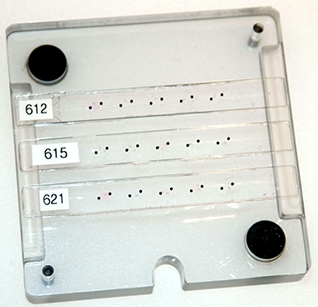
\includegraphics[width=2.5in]{./images/ace_m2_sample_tiles/platter_2104_web.png}
\caption{Sample platter 2104}
\end{center}
\end{figure}

\begin{figure}
\begin{center}
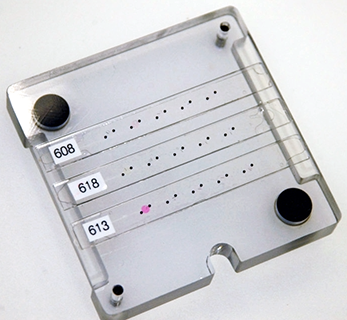
\includegraphics[width=2.5in]{./images/ace_m2_sample_tiles/platter_2105_web.png}
\caption{Sample platter 2105}
\end{center}
\end{figure}

The sample composition chart can be tedious to work with, because it's
effectively just a list of numbers. So to facilitate keeping track of the
different samples and their well locations, I created an icon-based chart. Each
entry in the table has a square icon tile, containing all of the relevant
information on each sample, which can be read at a quick glance.

\subsection{Dye samples}\label{dye-samples}
Dye samples have the name of the dye written in the color of the dye solution
(red and yellow), within the grey circle; the brightest colors represent the
higher concentration (of two), and the faded / lower-saturation text occurs in
samples with the lower concentrations.

\subsection{Colloidal suspensions}\label{colloidal-suspensions}
Each sample has a pie chart showing the volume fraction (out of 100\%) in bright
red. The radius of the circle denotes the particle size. Samples with the larger
(of two) particle diameters have circles that nearly fill the black squares,
where the exact volume fraction is written in text \emph{within} the pie chart.
For samples with the smaller particle diameter, the pie chart is substantially
smaller, and the text indicating the volume fraction resides \emph{outside} the
pie chart.

\subsection{Colloid-polymer mixtures}\label{colloid-polymer-mixtures}
These samples follow the same convention as for the colloidal suspensions;
however, those samples with depletant polymer have a blue triangle at the
lower-right of the square. For samples that are expected to phase separate in a
thermodynamic process known as spinodal decomposition, the blue triangle is
hatched. For samples that are supposed to kinetically arrest into a gel state,
the blue triangle is solid.

\begin{table*}
\begin{center}
\begin{tabular}{cccccc}
Strip & Well 1 & Well 2 & Well 3 & Well 4 & Well 5\\
\hline
\textbf{612} & 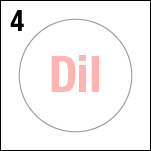
\includegraphics{./images/ace_m2_sample_tiles/sample04.png} & 
\includegraphics{./images/ace_m2_sample_tiles/sample06.png} & 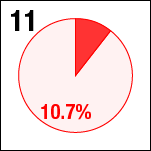
\includegraphics{./images/ace_m2_sample_tiles/sample11.png} & 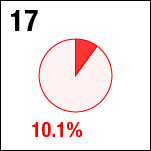
\includegraphics{./images/ace_m2_sample_tiles/sample17.png} & 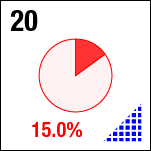
\includegraphics{./images/ace_m2_sample_tiles/sample20.png}\\
\textbf{615} & 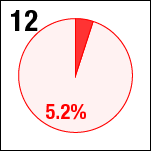
\includegraphics{./images/ace_m2_sample_tiles/sample12.png} & 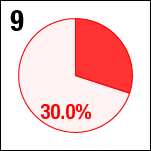
\includegraphics{./images/ace_m2_sample_tiles/sample09.png} & 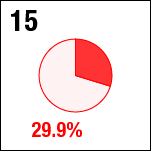
\includegraphics{./images/ace_m2_sample_tiles/sample15.png} & 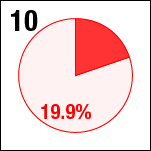
\includegraphics{./images/ace_m2_sample_tiles/sample10.png} & 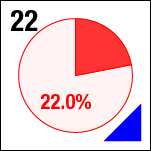
\includegraphics{./images/ace_m2_sample_tiles/sample22.png}\\
\textbf{621} & 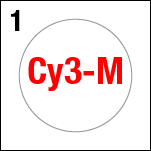
\includegraphics{./images/ace_m2_sample_tiles/sample01.png} & 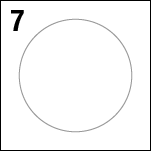
\includegraphics{./images/ace_m2_sample_tiles/sample07.png} & 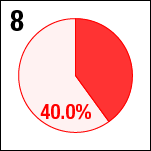
\includegraphics{./images/ace_m2_sample_tiles/sample08.png} & 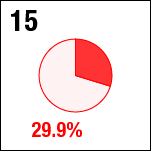
\includegraphics{./images/ace_m2_sample_tiles/sample15.png} & 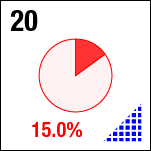
\includegraphics{./images/ace_m2_sample_tiles/sample20.png}\\
\end{tabular}
\caption{Sample platter 2104}
\end{center}
\end{table*}


\begin{table*}
\begin{center}
\begin{tabular}{cccccc}
Strip & Well 1 & Well 2 & Well 3 & Well 4 & Well 5\\
\hline
\textbf{608} & 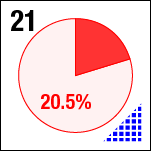
\includegraphics{./images/ace_m2_sample_tiles/sample21.png} & 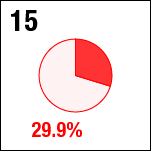
\includegraphics{./images/ace_m2_sample_tiles/sample15.png} & 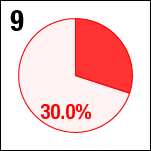
\includegraphics{./images/ace_m2_sample_tiles/sample09.png} & 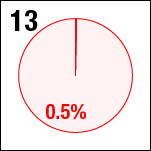
\includegraphics{./images/ace_m2_sample_tiles/sample13.png} & 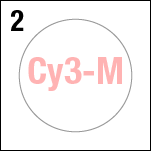
\includegraphics{./images/ace_m2_sample_tiles/sample02.png}\\
\textbf{618} & 
\includegraphics{./images/ace_m2_sample_tiles/sample05.png} & 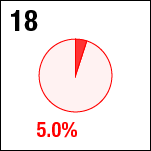
\includegraphics{./images/ace_m2_sample_tiles/sample18.png} & 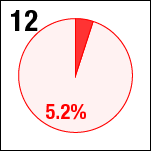
\includegraphics{./images/ace_m2_sample_tiles/sample12.png} & 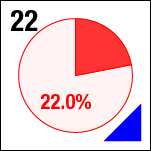
\includegraphics{./images/ace_m2_sample_tiles/sample22.png} & 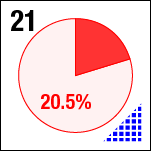
\includegraphics{./images/ace_m2_sample_tiles/sample21.png}\\
\textbf{613} & 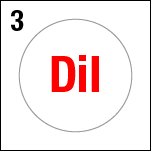
\includegraphics{./images/ace_m2_sample_tiles/sample03.png} & 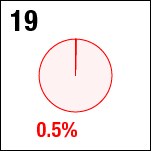
\includegraphics{./images/ace_m2_sample_tiles/sample19.png} & 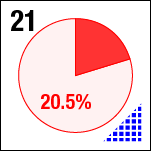
\includegraphics{./images/ace_m2_sample_tiles/sample21.png} & 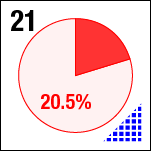
\includegraphics{./images/ace_m2_sample_tiles/sample21.png} & 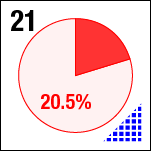
\includegraphics{./images/ace_m2_sample_tiles/sample21.png}\\
\end{tabular}
\caption{Sample platter 2105}
\end{center}
\end{table*}

\clearpage